% ============================================================
% Question Bank: ch06-06 Angle Relationships
% Topic Title: Angle Relationships: Supplementary, Complementary, and Vertical Angles
% CCSS: 7.G.B.5
% Questions: 30 (18 MC + 7 SA + 5 Graphical)
% ============================================================

% --- Multiple Choice Questions (18) ---

\begin{practiceQuestion}{6-6-q01}{mc}
\begin{questionText}
Two angles are supplementary. One angle is $115°$. What is the other angle?
\end{questionText}
\choiceA{$25°$}
\choiceB{$55°$}
\choiceC{$65°$}
\choiceD{$75°$}
\correctAnswer{C}
\explanation{Supplementary angles sum to $180°$. $180° - 115° = 65°$.}
\end{practiceQuestion}

\begin{practiceQuestion}{6-6-q02}{mc}
\begin{questionText}
Two angles are complementary. One angle is $27°$. What is the other angle?
\end{questionText}
\choiceA{$53°$}
\choiceB{$63°$}
\choiceC{$73°$}
\choiceD{$153°$}
\correctAnswer{B}
\explanation{Complementary angles sum to $90°$. $90° - 27° = 63°$.}
\end{practiceQuestion}

\begin{practiceQuestion}{6-6-q03}{mc}
\begin{questionText}
Two vertical angles are formed by intersecting lines. One angle is $72°$. What is the vertical angle?
\end{questionText}
\choiceA{$18°$}
\choiceB{$72°$}
\choiceC{$108°$}
\choiceD{$288°$}
\correctAnswer{B}
\explanation{Vertical angles are always equal. If one is $72°$, the vertical angle is also $72°$.}
\end{practiceQuestion}

\begin{practiceQuestion}{6-6-q04}{mc}
\begin{questionText}
Two supplementary angles are $(2x + 10)°$ and $(3x)°$. What is the value of $x$?
\end{questionText}
\choiceA{$30$}
\choiceB{$34$}
\choiceC{$36$}
\choiceD{$40$}
\correctAnswer{B}
\explanation{$2x + 10 + 3x = 180$. Combine: $5x + 10 = 180$. Subtract $10$: $5x = 170$. Divide: $x = 34$.}
\end{practiceQuestion}

\begin{practiceQuestion}{6-6-q05}{mc}
\begin{questionText}
Two complementary angles are $(x + 15)°$ and $(2x)°$. Find the smaller angle.
\end{questionText}
\choiceA{$25°$}
\choiceB{$40°$}
\choiceC{$50°$}
\choiceD{$65°$}
\correctAnswer{B}
\explanation{$x + 15 + 2x = 90$. Combine: $3x + 15 = 90$. Solve: $3x = 75$, $x = 25$. Angles: $25 + 15 = 40°$ and $2(25) = 50°$. The smaller is $40°$.}
\end{practiceQuestion}

\begin{practiceQuestion}{6-6-q06}{mc}
\begin{questionText}
Which pair of angles are supplementary?
\end{questionText}
\choiceA{$45°$ and $45°$}
\choiceB{$60°$ and $30°$}
\choiceC{$110°$ and $70°$}
\choiceD{$100°$ and $100°$}
\correctAnswer{C}
\explanation{Supplementary angles sum to $180°$. $110 + 70 = 180$ \checkmark. The others: $45 + 45 = 90$, $60 + 30 = 90$, $100 + 100 = 200$. Only C works.}
\end{practiceQuestion}

\begin{practiceQuestion}{6-6-q07}{mc}
\begin{questionText}
Two vertical angles are $(5x - 20)°$ and $(3x + 10)°$. What is the measure of each angle?
\end{questionText}
\choiceA{$45°$}
\choiceB{$55°$}
\choiceC{$60°$}
\choiceD{$75°$}
\correctAnswer{B}
\explanation{Vertical angles are equal: $5x - 20 = 3x + 10$. Subtract $3x$: $2x - 20 = 10$. Add $20$: $2x = 30$. Divide: $x = 15$. Angle: $5(15) - 20 = 55°$.}
\end{practiceQuestion}

\begin{practiceQuestion}{6-6-q08}{mc}
\begin{questionText}
An angle measures $38°$. Its complement measures:
\end{questionText}
\choiceA{$38°$}
\choiceB{$52°$}
\choiceC{$142°$}
\choiceD{$322°$}
\correctAnswer{B}
\explanation{Complementary angles sum to $90°$. $90° - 38° = 52°$.}
\end{practiceQuestion}

\begin{practiceQuestion}{6-6-q09}{mc}
\begin{questionText}
An angle is $4$ times its supplement. What is the angle?
\end{questionText}
\choiceA{$36°$}
\choiceB{$45°$}
\choiceC{$120°$}
\choiceD{$144°$}
\correctAnswer{D}
\explanation{Let the supplement be $x$. The angle is $4x$. Sum: $x + 4x = 180$. So $5x = 180$ and $x = 36°$. The angle: $4(36) = 144°$.}
\end{practiceQuestion}

\begin{practiceQuestion}{6-6-q10}{mc}
\begin{questionText}
Two angles are supplementary. One is $25°$ more than the other. What are the two angles?
\end{questionText}
\choiceA{$65°$ and $115°$}
\choiceB{$77.5°$ and $102.5°$}
\choiceC{$80°$ and $100°$}
\choiceD{$75°$ and $105°$}
\correctAnswer{B}
\explanation{Let the smaller be $x$. Then $x + (x + 25) = 180$. Combine: $2x + 25 = 180$. Solve: $2x = 155$, $x = 77.5°$. The other: $77.5 + 25 = 102.5°$.}
\end{practiceQuestion}

\begin{practiceQuestion}{6-6-q11}{mc}
\begin{questionText}
Which statement about vertical angles is always true?
\end{questionText}
\choiceA{They are supplementary}
\choiceB{They are complementary}
\choiceC{They are equal}
\choiceD{They sum to $360°$}
\correctAnswer{C}
\explanation{Vertical angles are always equal. They are formed by two intersecting lines, and the opposite angles are congruent.}
\end{practiceQuestion}

\begin{practiceQuestion}{6-6-q12}{mc}
\begin{questionText}
An angle and its complement are in the ratio $1:4$. What is the larger angle?
\end{questionText}
\choiceA{$18°$}
\choiceB{$36°$}
\choiceC{$72°$}
\choiceD{$90°$}
\correctAnswer{C}
\explanation{Let the angles be $x$ and $4x$. Sum: $x + 4x = 90$. So $5x = 90$ and $x = 18$. The larger angle: $4(18) = 72°$.}
\end{practiceQuestion}

\begin{practiceQuestion}{6-6-q13}{mc}
\begin{questionText}
Two lines intersect. One angle formed is $130°$. What are the measures of all four angles?
\end{questionText}
\choiceA{$130°$, $130°$, $50°$, $50°$}
\choiceB{$130°$, $50°$, $130°$, $100°$}
\choiceC{$130°$, $130°$, $130°$, $130°$}
\choiceD{$130°$, $60°$, $130°$, $40°$}
\correctAnswer{A}
\explanation{Vertical angles are equal ($130°$ and $130°$). Adjacent angles are supplementary: $180° - 130° = 50°$. The four angles are $130°$, $50°$, $130°$, $50°$.}
\end{practiceQuestion}

\begin{practiceQuestion}{6-6-q14}{mc}
\begin{questionText}
Angles $A$ and $B$ are complementary. Angle $A$ is $(3x - 5)°$ and angle $B$ is $(x + 15)°$. What is angle $A$?
\end{questionText}
\choiceA{$20°$}
\choiceB{$35°$}
\choiceC{$55°$}
\choiceD{$65°$}
\correctAnswer{C}
\explanation{$3x - 5 + x + 15 = 90$. Combine: $4x + 10 = 90$. Solve: $4x = 80$, $x = 20$. Angle $A$: $3(20) - 5 = 55°$.}
\end{practiceQuestion}

\begin{practiceQuestion}{6-6-q15}{mc}
\begin{questionText}
Which pair of angles is complementary?
\end{questionText}
\choiceA{$50°$ and $130°$}
\choiceB{$55°$ and $35°$}
\choiceC{$60°$ and $60°$}
\choiceD{$45°$ and $135°$}
\correctAnswer{B}
\explanation{Complementary angles sum to $90°$. Only $55 + 35 = 90$.}
\end{practiceQuestion}

\begin{practiceQuestion}{6-6-q16}{mc}
\begin{questionText}
Two supplementary angles are equal. What is the measure of each?
\end{questionText}
\choiceA{$45°$}
\choiceB{$60°$}
\choiceC{$90°$}
\choiceD{$180°$}
\correctAnswer{C}
\explanation{If two equal angles sum to $180°$, then each is $180 \div 2 = 90°$.}
\end{practiceQuestion}

\begin{practiceQuestion}{6-6-q17}{mc}
\begin{questionText}
An angle is $12°$ less than its complement. What is the angle?
\end{questionText}
\choiceA{$39°$}
\choiceB{$42°$}
\choiceC{$48°$}
\choiceD{$51°$}
\correctAnswer{A}
\explanation{Let the angle be $x$ and its complement be $x + 12$. Sum: $x + (x + 12) = 90$. Combine: $2x + 12 = 90$. Solve: $2x = 78$, $x = 39°$.}
\end{practiceQuestion}

\begin{practiceQuestion}{6-6-q18}{mc}
\begin{questionText}
Adjacent angles on a straight line must sum to:
\end{questionText}
\choiceA{$90°$}
\choiceB{$180°$}
\choiceC{$270°$}
\choiceD{$360°$}
\correctAnswer{B}
\explanation{A straight line measures $180°$. Adjacent angles that together form a straight line must sum to $180°$ (they are supplementary).}
\end{practiceQuestion}

% --- Short Answer Questions (7) ---

\begin{practiceQuestion}{6-6-q19}{sa}
\begin{questionText}
Find the complement of $67°$.
\end{questionText}
\correctAnswer{$23°$}
\explanation{$90° - 67° = 23°$.}
\end{practiceQuestion}

\begin{practiceQuestion}{6-6-q20}{sa}
\begin{questionText}
Find the supplement of $43°$.
\end{questionText}
\correctAnswer{$137°$}
\explanation{$180° - 43° = 137°$.}
\end{practiceQuestion}

\begin{practiceQuestion}{6-6-q21}{sa}
\begin{questionText}
Two vertical angles are $(7x + 1)°$ and $(5x + 13)°$. Find $x$ and the angle measure.
\end{questionText}
\correctAnswer{$x = 6$; the angles are $43°$}
\explanation{Vertical angles are equal: $7x + 1 = 5x + 13$. Subtract $5x$: $2x + 1 = 13$. Subtract $1$: $2x = 12$. Divide: $x = 6$. Angle: $7(6) + 1 = 43°$.}
\end{practiceQuestion}

\begin{practiceQuestion}{6-6-q22}{sa}
\begin{questionText}
Two supplementary angles are in the ratio $5:4$. Find both angles.
\end{questionText}
\correctAnswer{$100°$ and $80°$}
\explanation{$5x + 4x = 180$. Combine: $9x = 180$. Solve: $x = 20$. Angles: $5(20) = 100°$ and $4(20) = 80°$.}
\end{practiceQuestion}

\begin{practiceQuestion}{6-6-q23}{sa}
\begin{questionText}
An angle is $3$ times its complement. Find the angle.
\end{questionText}
\correctAnswer{$67.5°$}
\explanation{Let complement be $x$. Angle $= 3x$. Sum: $x + 3x = 90$. So $4x = 90$ and $x = 22.5°$. The angle: $3(22.5) = 67.5°$.}
\end{practiceQuestion}

\begin{practiceQuestion}{6-6-q24}{sa}
\begin{questionText}
Three angles meet at a point on a line: $50°$, $(2x + 10)°$, and $x°$. Find $x$.
\end{questionText}
\correctAnswer{$40$}
\explanation{Angles on a line sum to $180°$: $50 + 2x + 10 + x = 180$. Combine: $3x + 60 = 180$. Solve: $3x = 120$, $x = 40$.}
\end{practiceQuestion}

\begin{practiceQuestion}{6-6-q25}{sa}
\begin{questionText}
Two lines intersect. One of the four angles is $(4x + 20)°$. Its adjacent angle is $(6x - 10)°$. Find the value of $x$.
\end{questionText}
\correctAnswer{$17$}
\explanation{Adjacent angles at an intersection are supplementary: $4x + 20 + 6x - 10 = 180$. Combine: $10x + 10 = 180$. Solve: $10x = 170$, $x = 17$.}
\end{practiceQuestion}

% --- Graphical Questions (3 GMC + 2 GSA) ---

\begin{practiceQuestion}{6-6-q26}{gmc}
\begin{questionText}
Two lines intersect as shown. What is the value of $x$?

\begin{center}
\begin{tikzpicture}[scale=0.8]
  \draw[thick] (-3,0) -- (3,0);
  \draw[thick] (-2,-2) -- (2,2);
  \node at (1.5,0.5) {\small $x°$};
  \node at (-1.5,-0.6) {\small $x°$};
  \node at (-1.2,0.8) {\small $135°$};
\end{tikzpicture}
\end{center}
\end{questionText}
\choiceA{$35°$}
\choiceB{$45°$}
\choiceC{$55°$}
\choiceD{$135°$}
\correctAnswer{B}
\explanation{The angle $x°$ and $135°$ are supplementary (they are adjacent on a straight line): $x + 135 = 180$. So $x = 45°$.}
\end{practiceQuestion}

\begin{practiceQuestion}{6-6-q27}{gmc}
\begin{questionText}
In the diagram below, lines $AB$ and $CD$ intersect at point $O$. Find the value of $y$.

\begin{center}
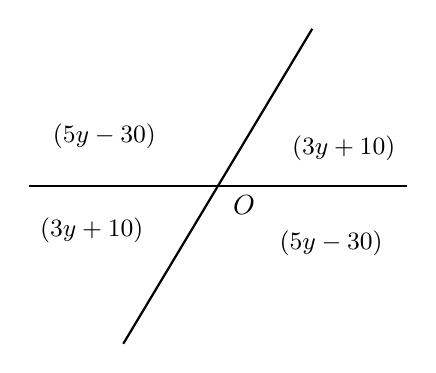
\begin{tikzpicture}[scale=0.8]
  \draw[thick] (-3,0) -- (3,0);
  \draw[thick] (-1.5,-2.5) -- (1.5,2.5);
  \node at (0,0) [below right,xshift=2pt] {$O$};
  \node at (2,0.6) {\small $(3y + 10)°$};
  \node at (-2,-0.7) {\small $(3y + 10)°$};
  \node at (-1.8,0.8) {\small $(5y - 30)°$};
  \node at (1.8,-0.9) {\small $(5y - 30)°$};
\end{tikzpicture}
\end{center}
\end{questionText}
\choiceA{$10$}
\choiceB{$20$}
\choiceC{$25$}
\choiceD{$35$}
\correctAnswer{C}
\explanation{Adjacent angles are supplementary: $(3y + 10) + (5y - 30) = 180$. Combine: $8y - 20 = 180$. Solve: $8y = 200$, $y = 25$.}
\end{practiceQuestion}

\begin{practiceQuestion}{6-6-q28}{gmc}
\begin{questionText}
In the diagram, angle $1$ and angle $2$ are complementary. Angle $1$ measures $53°$. What is angle $2$?

\begin{center}
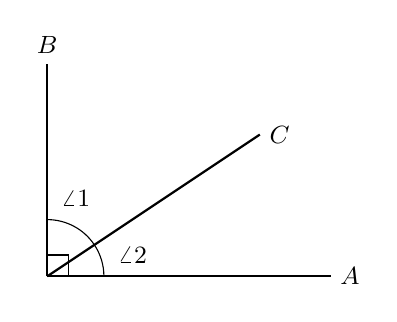
\begin{tikzpicture}[scale=0.9]
  \draw[thick] (0,0) -- (4,0);
  \draw[thick] (0,0) -- (0,3);
  \draw[thick] (0,0) -- (3,2);
  \draw (0.8,0) arc[start angle=0,end angle=34,radius=0.8];
  \node at (1.2,0.3) {\small $\angle 2$};
  \draw (0,0.8) arc[start angle=90,end angle=34,radius=0.8];
  \node at (0.4,1.1) {\small $\angle 1$};
  \node[right] at (4,0) {\small $A$};
  \node[above] at (0,3) {\small $B$};
  \node[right] at (3,2) {\small $C$};
  % Right angle mark
  \draw (0.3,0) -- (0.3,0.3) -- (0,0.3);
\end{tikzpicture}
\end{center}
\end{questionText}
\choiceA{$27°$}
\choiceB{$37°$}
\choiceC{$53°$}
\choiceD{$127°$}
\correctAnswer{B}
\explanation{The two angles together form a right angle ($90°$). $90° - 53° = 37°$.}
\end{practiceQuestion}

\begin{practiceQuestion}{6-6-q29}{gsa}
\begin{questionText}
Two lines intersect as shown. Find the values of $a$, $b$, and $c$.

\begin{center}
\begin{tikzpicture}[scale=0.8]
  \draw[thick] (-3,0) -- (3,0);
  \draw[thick] (-2,-2.5) -- (2,2.5);
  \node at (1.8,0.7) {\small $a°$};
  \node at (-1.8,0.7) {\small $b°$};
  \node at (-1.8,-0.8) {\small $c°$};
  \node at (1.8,-0.8) {\small $52°$};
\end{tikzpicture}
\end{center}
\end{questionText}
\correctAnswer{$a = 128°$, $b = 52°$, $c = 128°$}
\explanation{Vertical to $52°$: $b = 52°$. Supplementary to $52°$: $a = 180° - 52° = 128°$. Vertical to $a$: $c = 128°$.}
\end{practiceQuestion}

\begin{practiceQuestion}{6-6-q30}{gsa}
\begin{questionText}
In the figure below, three angles meet on a straight line. Find the value of $x$ and the measure of each angle.

\begin{center}
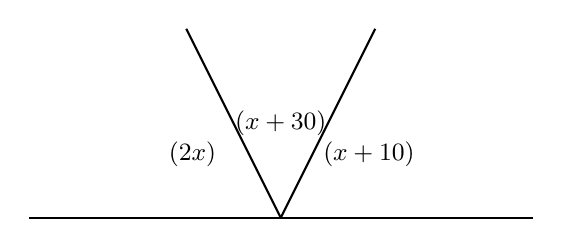
\begin{tikzpicture}[scale=0.8]
  \draw[thick] (-4,0) -- (4,0);
  \draw[thick] (0,0) -- (-1.5,3);
  \draw[thick] (0,0) -- (1.5,3);
  \node at (-1.4,1) {\small $(2x)°$};
  \node at (0,1.5) {\small $(x + 30)°$};
  \node at (1.4,1) {\small $(x + 10)°$};
\end{tikzpicture}
\end{center}
\end{questionText}
\correctAnswer{$x = 35$; angles are $70°$, $65°$, and $45°$}
\explanation{Angles on a line sum to $180°$: $2x + (x + 30) + (x + 10) = 180$. Combine: $4x + 40 = 180$. Solve: $4x = 140$, $x = 35$. Angles: $2(35) = 70°$, $35 + 30 = 65°$, $35 + 10 = 45°$. Check: $70 + 65 + 45 = 180°$ \checkmark.}
\end{practiceQuestion}
